%!TEX root = ../thesis.tex
\chapter{Background}
\label{ch:background}

This thesis uses newly developed approaches from applied topology to study open problems in evolutionary biology and genomics.
Here we supply sufficient background to motivate our approach
Exposition for specific applications can be found in their respective individual chapters.

\section{Biology}

In this section we present a basic introduction to molecular sequence data: what the data looks like, the processes by which it is generated, and the phylogenetic methods by which it is analyzed.

\subsection{Genes and Genomes}

The information required to express an organism's biological form and function is contained in the genome, the complete sequence of nucleotides (DNA) contained in every cell\footnote{While often represented as a linear string of characters, this representation can be misleading, as many organisms, primarily viruses and bacteria, have circular genomes.}
Embedded in this sequence are subsequences representing genes, which code for the protein products


Embedded in the genome is a complex regulatory pattern of transcription factors controlling the expression of particular genes controlling cell differentiation and development.
that controls the differential expression of particular 
Embedded in this sequence is a complex regulatory pattern of transcription factors controlling the expression of particular genes.

\kje{Include a figure of a gene / genome?}
Following the central dogma of biology, DNA is transcribed into RNA, RNA is translated into amino acids, and amino acids are folded into proteins \cite{Crick:1970wb}.
Proteins comprise the functional unit of biology.

Beyond simply coding for function, the genome includes an imprint of the evolutionary history that gave rise to the organism.
By comparing the genomes of multiple organisms, inferences can be drawn about the evolutionary relationships among extant organisms as well as the processes that generated the observed diversity.
The field concerned with exploring these relationships is \emph{comparative genomics}.

\subsection{Evolutionary Processes}

Evolution describes the gradual change in phenotypes arising from random variation and subject to natural selection.
The processes giving rise to diversity can be classified into two categories: clonal and reticulate.

\subsubsection{Clonal Evolution}

Clonal evolution is the process of reproduction whereby genetic material is transferred directly from parent to offspring.
Population diversity is generated by stochastic mutation and maintained over multiple generations by random drift.

It is clonal evolution that Darwin had in mind when he described the idea of descent with modification, whereby a parent passes genomic information to an offspring subject to random drift.
Importantly, because there is always a direct parent--offspring relationship, clonal evolution will be consistent with a phylogenetic tree model.

\subsubsection{Reticulate Evolution}

Reticulate evolution, or horizontal evolution, refers to exchange or acquisition of genetic material via processes that do not reflect a direct parent--offspring relationship.
As we will see, these processes can make inferences of evolutionary relationships difficult.
Different reticulate processes occur in different types of organisms (summarized in Table \ref{table:reticulation_processes}).

In viruses, reticulation can occur when two virus particles coinfect the same host cell.
In the process of replicating, the viruses can exchange genetic material in one of two ways: reassortment and recombination (the two processes are contrasted in Figure~\ref{fig:viral_reticulation}).
Reassortment occurs in viruses whose genomes are structured into distinct segments, such as influenza.
Segments can be thought of as chromosomes.
Viral replication involves the packaging of each segment of the virus, and in the presence of coinfection segments from different virus particles can exchange.
Recombination occurs in nonsegmented virusesm, such as HIV, and involves intrasegmental crossover.
Intrasegmental crossover is a type of \emph{homologous recombination}.
Reassortment, on the other hand, is a type of \emph{nonhomologous recombination}.

\begin{figure}
\centering
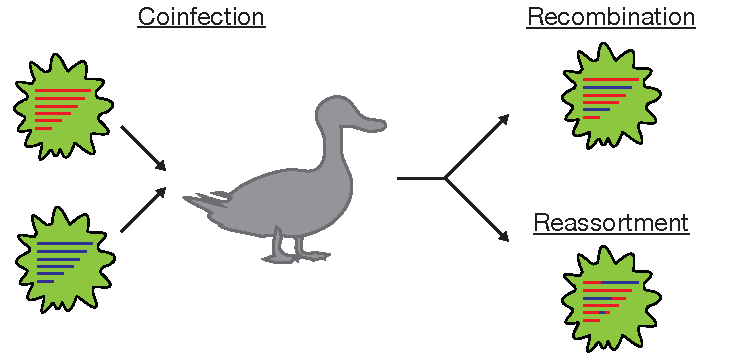
\includegraphics[]{./fig/background/viral_reticulation.pdf}
\caption[Viral recombination and reassortment]{The two modes of viral reticulation. Coinfection of the same host cell can lead to either reassortment, where whole viral segments are exchanged, or recombination, in which breakpoints can occur within segments. The former process is common in influenza, the latter in HIV. The end result, however, is }
\label{fig:viral_reticulation}
\end{figure}

In bacteria, reticulation can often involve the direct exchange of genes.
Reticulation is often called horizontal gene transfer or lateral gene transfer.
Horizontal exchange occurs when a donor bacteria transmits foreign DNA into a genetically distinct bacteria strain.
Three mechanisms of horizontal transfer are identified, depending on the route by which foreign DNA is acquired \cite{Ochman:2000dr}.
Foreign DNA can be acquired via uptake from an external environment (transformation), via viral-mediated processes (transduction), or via direct cell-to-cell contact between bacterial strains (conjugation).

In eukaryotes, several reticulation processes 

\footnote{One might wonder about sexual reproduction -- a descendent can be seen as a hybridization of both mother and father. Indeed, sexual reproduction can itself be considered a form of reticulate evolution. In the case of \emph{H. sapiens}, a diploid species with two copies of each chromosome, XXX. However, from an evolutionary perspective, the process can be decoupled into two independent clonal processes. When discussing the human species, researchers will commonly refer to the most recent common ancestor on the patrilineal as Y-chromosomal Adam and the most recent common ancestor on the matrilineal as mitochondrial Eve.}

In eukaryotes: hybridization and meiotic recombination.
Patterns of meiotic recombination can be 

\begin{tabularx}{\textwidth}{lll}
\toprule
Organism & Process & Description \\
\midrule
\multirow{2}{*}{Virus} & Reassortment & INSERT FIGURE \\
                       & Recombination & INSERT FIGURE \\
\midrule
\multirow{3}{*}{Bacteria} & Transformation & xx \\
                          & Transduction   & xx \\
                          & Conjugation    & xx \\
\midrule
\multirow{2}{*}{Eukaryotes} & Meiotic Recombination & Description \\
                            & Hybridization         & Description \\
\bottomrule
\label{table:reticulation_processes}
\end{tabularx}

The presence of horizontal gene transfer in a set of organisms can be most clearly identified by comparing the phylogenetic trees built from different genes.
If horizontal gene transfer has occurred, the set of \emph{gene trees} will reflect different evolutionary relationships and not be consistent with a single tree topology.
A subfield of comparative genomics is concerned with building \emph{species trees} from sets of gene trees, however in the case where there is substantial disagreement among gene trees the very notion of a species tree may be flawed.

Traditionally, evolutionary biology has concerned itself with characterizing relationships in light of vertical evolution alone.
However, increasing evidence \kje{(what evidence?)} has pointed to the important role played by horizontal evolution, particularly in prokaryotic evolution.
\kje{[Further citations and exposition of Doolittle, Koonin, and Gogarten.]}

\subsection{Mathematical Models of Evolution}

Mathematical population genetics is concerned with properties of populations as they are subject to evolutionary forces over long time scales.
These forces include natural selection, genetic drift, mutation, and recombination.
Historically the input data for population genetics models was comparative studies of allele frequencies across populations.
These studies have primarily been replaced by large-scale genomic surveys which have provided unprecedented insight into ancient population structure and historical migrations.
\kje{[Give an example and cite work of reich / bustamente, etc.]}

Incorporate understanding of real data
These models allow two things: 1) simulate genomic data under realistic processes and 2) build statistical models to estimate biological parameters from real data.

\subsubsection{The Wright-Fisher Model}

The Wright-Fischer model is a forward time simulation of an evolving population.
In the simplest case, the model describes neutral evolution of a constant population size with no structure and constant genome length.
The model proceeds in units of generations.
At each generation, a member of the population is an offspring of a randomly selected ancestor from the previous generation.
This offspring inherits its ancestors genomes, with mutations introduced at some base rate $\mu$.
A member of previous generation with no offspring will be considered extinct.
\kje{[Figure comparing Wright-Fisher and Coalescent.]}

\subsubsection{The Coalescent Process}

The coalescent process is a stochastic model that generates the genealogy of individuals sampled from an evolving population \cite{Wakeley:2009}.
The genealogy is then used to simulate the genetic sequences of the sample.
This model is essential to many methods commonly used in population genetics.
Starting with a present-day sample of $n$ individuals, each individual's lineage is traced backward in time, towards a mutual common ancestor.
Two separate lineages collapse via a coalescence event, representing the sharing of an ancestor by the two lineages.
The stochastic process ends when all lineages of all sampled individuals collapse into a single common ancestor.
In this process, if the total (diploid) population size $N$ is sufficiently large, then the expected time before a coalescence event, in units of $2N$ generations, is approximately exponentially distributed:
\begin{equation}
P(T_{k}=t) \approx \binom{k}{2} e^{-\binom{k}{2} t},
\end{equation}
where $T_k$ is the time that it takes for $k$ individual lineages to collapse into $k-1$ lineages.

After generating a genealogy, the genetic sequences of the sample can be simulated by placing mutations on the individual branches of the lineage.
The number of mutations on each branch is Poisson-distributed with mean $\theta t / 2$, where $t$ is the branch length and $\theta$ is the population-scaled mutation rate.
In this model, the average \emph{genetic distance} between any two sampled individuals, defined by the number of mutations separating them, is $\theta$.

The coalescent with recombination is an extension of this model that allows different genetic loci to have different genealogies.
Looking backward in time, recombination is modeled as a splitting event, occurring at a rate determined by population-scaled recombination rate $\rho$, such that an individual has a different ancestor at different loci.
Evolutionary histories are no longer represented by a tree, but rather by an \emph{ancestral recombination graph}.
Recombination is the component of the model generating nontrivial topology by introducing deviations from a contractibile tree structure, and is the component which we would like to quantify.
Coalescent simulations were performed using \texttt{ms} \cite{Hudson:2002}.

\subsubsection{Metrics on Sequeces}


What metrics can we put on aligned sequences?

For the sequences from different organisms to be compared, they must first be aligned.
A sequence alignment is an arrangement of the characters in a set of sequences into a set of columns such that characters sharing evolutionary identity are in the same column.
In this case insertion and deletions can introduce gaps.
Alignment can be a complex part of any sequence analysis, particularly when there is substantial divergence between sequences of interest.
Performing sequence alignment is largely beyond the scope of this thesis, and in general we assume sufficient sequence similarity such that alignment can be performed without difficulty.

The simplest model, and the one most commonly adopted in this thesis, is the Hamming metric, which simply counts the differences between two aligned sequences.

More biologically motivated metrics will incorporate some model of evolution and account for the possibility of back mutation.
These include Jukes-Cantor, Nei-Tamura, etc.
\kje{[Worth expanding?]}

Jukes-Cantor metric is defined as 
\begin{equation}
d=-\frac{3}{4}\ln(1-\frac{4}{3}p).
\end{equation}

\subsection{Phylogenetic Methods}

A phylogenetic tree is XXX.


Molecular phylogenetics refers to a large collection of methods for inferring evolutionary relationships among a set of species from molecular sequence data.
In practice, this 
In practice: tree-building.

Starting with a set of sequences that share some similarity, an alignment is performed.
The alignment allows columns of the sequence to be directly compared.
From an alignment, one can then directly use parsimony or likelihood approaches.
Alternatively, one can compute a matrix of pairwise distances and then construct a tree that best approximates these distances.
Most relevant to this thesis are the distance-based approaches (because they can be viewed as finite metric spaces amenable to topological analysis).
Only in the case of perfectly additive data will a tree be able to exactly fit the matrix.
\kje{(Define additivity -- four point condition.)}
Identifying a pairwise distance matrix with a finite metric space representation is a crucial step that allows most of the machinery described later to be applied.
\kje{Rooted vs unrooted.}

\subsubsection{Distance Matrix Methods}

Introduced by Cavalli-Sforza and Edwards in 1967 \cite{CavalliSforza:1967th} and Fitch and Margoliash in 1967 \cite{Fitch:1967we}.
Fitch-Margoliash method is a weighted least squares tree-fitting method (larger distances are weighted less, due to higher random error).
Compute a matrix of pairwise distances and then find the tree that best approximates those distances.
Neighbor joining is now the most commonly used distance-matrix approach because it can perfectly reconstruct an additive tree.
Neighbor joining was introduced by Saitou and Nei in 1987 \cite{Saitou:1987wo}.

Limitation: Distance methods do not make use of all of the information in the sequence.

\subsubsection{Phylogenetic Networks}

There are several existing methods for representing reticulate evolution.
Most of these methods generalize phylogenetic trees into \emph{phylogenetic networks}, which attempt to reconcile the presence of horizontal evolution in sequence data.
However, most simply present corrections to phylogenetic trees, which can fail in cases where horizontal evolution is pervasive, as in many prokaryote datasets.
Additionally, the resulting neteworks can be complex and difficult to interpret quantitatively.
\kje{[Expand. See Morrison review. Split Networks.]}

\subsubsection{Number of Tree Topologies}

The number of unrooted bifurcating tree topologies with $L$ leaves is $(2L-5)!!$.\footnote{The double factorial is defined as $n!!=n(n-2)(n-4)\cdots$.}
This can be easily shown using induction.
For $L=3$, we have $\mathcal{T}(3)=1$ and $3$ branches.
To pass to $L=4$, we can add the fourth leaf to any of the $3$ branches, resulting in $3$ different topologies.
For $L=4$, we have $\mathcal{T}(4)=3$.
Every time we add a leaf, we add two branches -- one external and one internal.
For $L=n$, we have $\mathcal{T}(n)=(2n-5)!!$ and $2n-3$ branches.
For $L=n+1$, we can add the new external branch to any of the current $2n-3$ branches.
A rooted tree with $L$ leaves can be considered as an unrooted tree with $L+1$ leaves.
Therefore, the number of rooted bifurcating tree topologies with $L$ leaves is $(2L-3)!!$
As can be seen, the number of tree topologies explodes with the number of leaves.
Fitch quote: \emph{more than 20 species, more than Avogadro's number of topologies.}

\subsubsection{Space of Phylogenetic Trees}

A phylogenetic tree is characterized by its number of leaves, the particular tree topology, and the length of each branch.
Tree space refers to an abstract construction that represents each possible tree as a point in a geometric space.
Abstract studies of tree space were initiated by Billera, Holmes, and Vogtmann (BHV) in \cite{Billera:2001tv}.

In the BHV model, each point represents an unrooted binary tree with $L$ leaves and strictly positive branch lengths.

Number of interior edges $r=L-3$, a particular additive tree can be plotted as a point in the positive open orthant $(0,\infty)^{r}$.

A single orthant corresponds to a single tree topology.

\begin{figure}
\centering
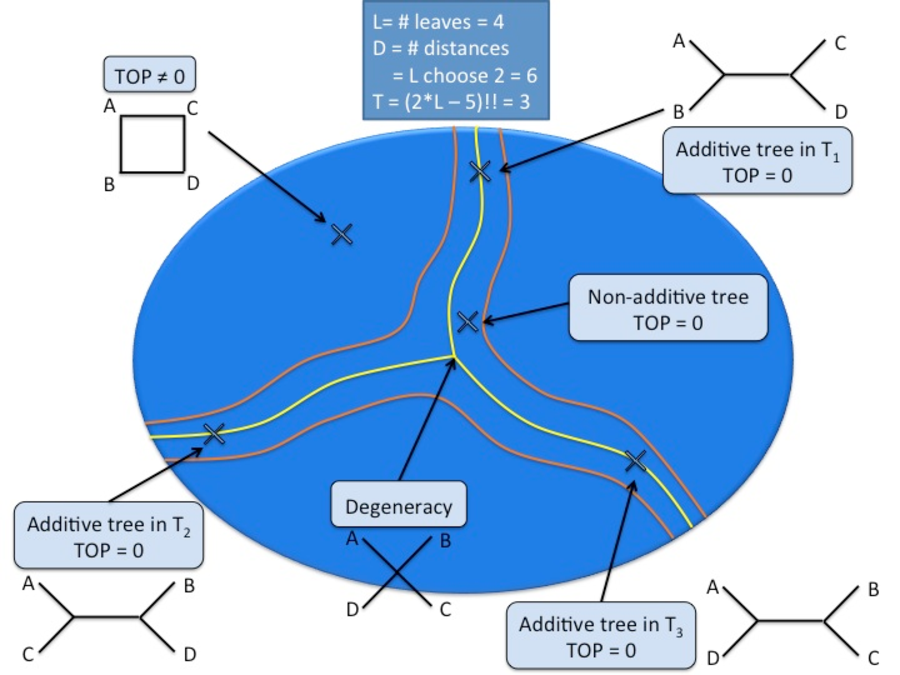
\includegraphics[]{./fig/TreeSpace.pdf}
\caption{Tree Space}
\label{background:fig:TreeSpace}
\end{figure}

